
\documentclass{beamer}

\usepackage[spanish]{babel}
\usepackage{graphicx,hyperref,ru,url}
\usepackage{graphicx}
\usepackage[utf8]{inputenc}
\usepackage{amsmath}
\usepackage{amsfonts}
\usepackage{amssymb}
\usepackage{lipsum}
\usepackage{ragged2e}
\usepackage{float}
% The title of the presentation:
%  - first a short version which is visible at the bottom of each slide;
%  - second the full title shown on the title slide;
\title[Licenciatura en Física]{Estimación y Evaluación de Eficiencia de Atenuación de Elementos de Protección Mediante Simulación en Geant4.}


% Optional: a subtitle to be dispalyed on the title slide
% \subtitle{En español}

% The author(s) of the presentation:
%  - again first a short version to be displayed at the bottom;
%  - next the full list of authors, which may include contact information;
\author[Isabel Alejandra Morales S.]{
  Isabel Alejandra Morales Salamanca \\\medskip
  {\small \url{iimoralezs@correo.udistrital.edu.co}}
 \\}

% The institute:
%  - to start the name of the university as displayed on the top of each slide
%    this can be adjusted such that you can also create a Dutch version
%  - next the institute information as displayed on the title slide
\institute[Universidad Distrital]{
  Instituto de Ingeominas -- Licenciatura en Física \\
  Universidad Distrital Francisco José de Caldas}

% Add a date and possibly the name of the event to the slides
%  - again first a short version to be shown at the bottom of each slide
%  - second the full date and event name for the title slide
% \date[slides Example 2010]{
%   the 1st example presentation 2010 \\
%   7th October 2010}

\begin{document}

\begin{frame}
  \titlepage
\end{frame}

\begin{frame}
  \frametitle{Contenido}
  

  \tableofcontents
\end{frame}

% Section titles are shown in at the top of the slides with the current section 
% highlighted. Note that the number of sections determines the size of the top 
% bar, and hence the university name and logo. If you do not add any sections 
% they will not be visible.
\section{Problema}

\begin{frame}
  \frametitle{Problema}

En el uso habitual de la radiación al interactuar con el paciente, una  parte de la radicación es absorbida, otra parte atraviesa el paciente y otra se dispersa en direcciones distintas (multidireccional). Existen efectos asociados a la radiación dispersa en otras direcciones%\cite{xxx}.
En condiciones normales%\cite{xxx}
la  radiación dispersa, justamente por el carácter que tiene de multidireccionalidad es la causa principal de la exposición a la  irradiación de los profesionales, trabajadores y público en general %\cite{xxx}.
En este trabajo evalúa la eficiencia de Atenuación de una prenda de protección radiológica (chaleco) a través de un laboratorio virtual. Se estudia el porcentaje de atenuación de la prenda protectora mediante los parámetros de: espesor y energía.

  %\begin{itemize}
   % \item This is just a short example
    %\item The comments in the \LaTeX\ file are most important
    %\item This is just the result after running pdflatex
    %\item The style is based on the webpage \url{http://www.ru.nl/}
  %\end{itemize}
\end{frame}


\section{Metodologia}
\begin{enumerate} 
 \item Revisión de antecedentes. 
\begin{center}
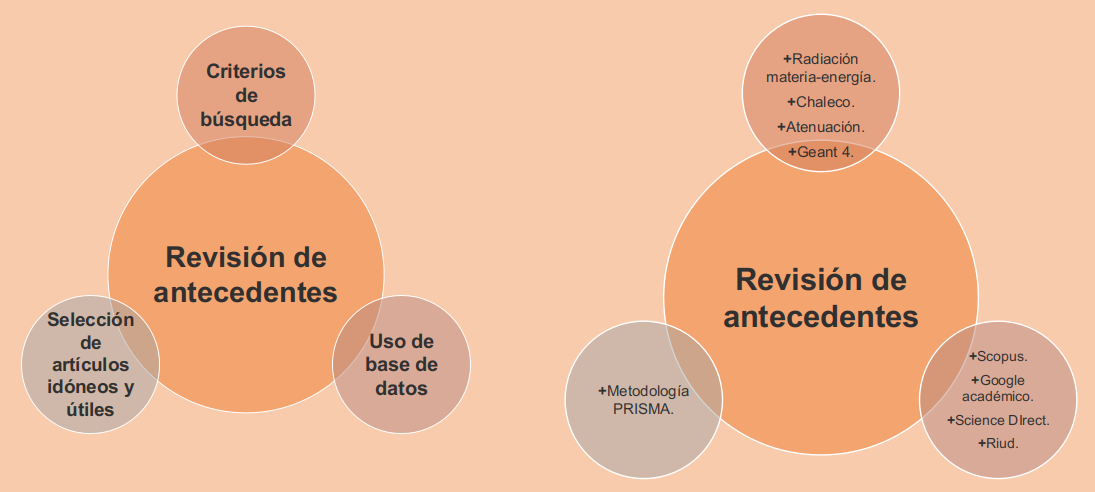
\includegraphics[width=10.3cm,height=7.9
cm]{T}
\end{center}
\newpage
\item Revisión de antecedentes. 
\begin{center}
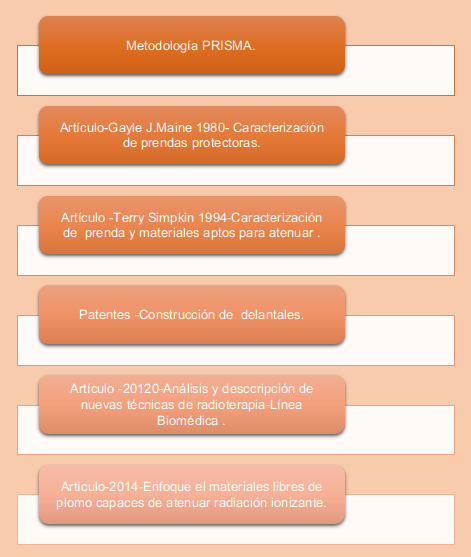
\includegraphics[width=9.7cm,height=7.7cm]{2T.png}
\end{center}
\newpage
\item Revisión de antecedentes. 
\begin{center}
\includegraphics[width=10cm,height=7.5cm]{3T}
\end{center}




\newpage
\item Demarcación de  principios físicos asociados a la solución del problema.
\begin{center}
\includegraphics[width=10cm,height=7cm]{4T}
\end{center}
\newpage
\item Demarcación de  principios físicos asociados a la solución del problema. 
\begin{center}
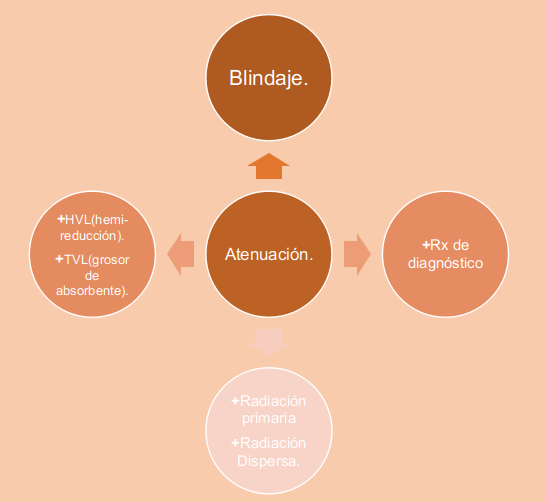
\includegraphics[width=10cm,height=7cm]{5T}
\end{center}
\newpage

\item Demarcación de  principios físicos asociados a la solución del problema. 
\begin{center}
\includegraphics[width=10cm,height=7cm]{6T}
\end{center}


\newpage
 \item Proponer modelo físico.
\begin{center}
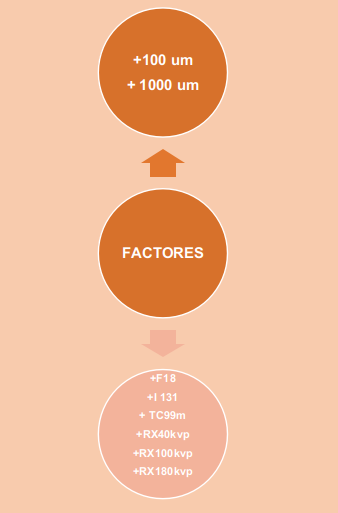
\includegraphics[width=5.5cm,height=7.5cm]{7T}
\end{center}
 
\newpage
 \item Proponer modelo físico. 
\begin{center}
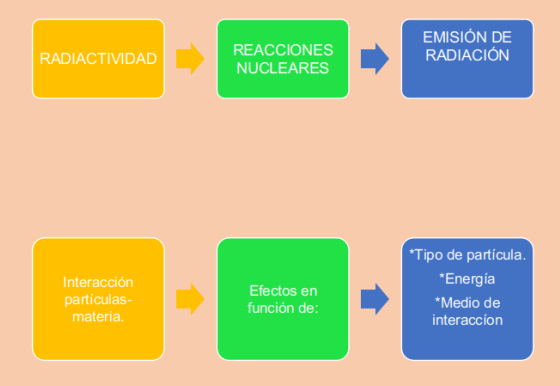
\includegraphics[width=9.5cm,height=7.5cm]{10T}
\end{center}
\newpage
 \item Proponer modelo físico.
\begin{center}
\includegraphics[width=10cm,height=7cm]{11T}
\end{center}
\newpage
 \item Proponer modelo físico.
\begin{center}
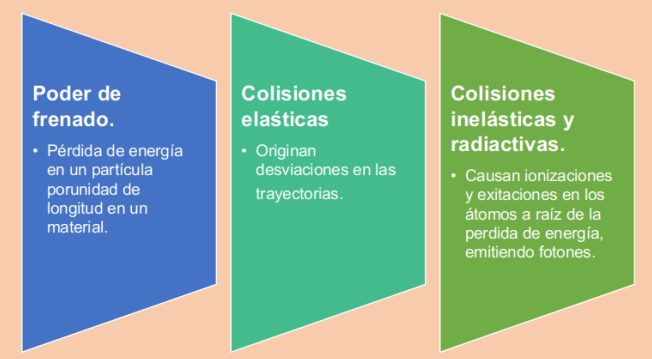
\includegraphics[width=10cm,height=7cm]{12T}
\end{center}
\newpage
 \item Proponer modelo físico.
 \begin{center}
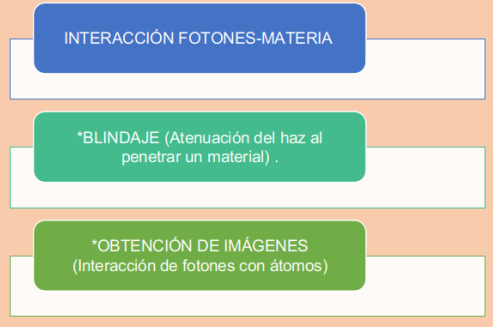
\includegraphics[width=10cm,height=7cm]{13T}
\end{center}
\newpage
 \item Proponer modelo físico.
\begin{center}
\includegraphics[width=10cm,height=7cm]{14T}
\end{center}
\newpage
 \item Proponer modelo físico.
\begin{center}
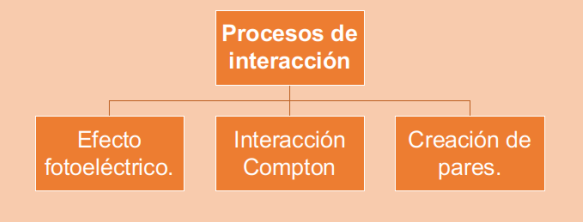
\includegraphics[width=10cm,height=7cm]{15T}
\end{center}



 \newpage
 \item Estructura metodologica para la simulación.
\begin{center}
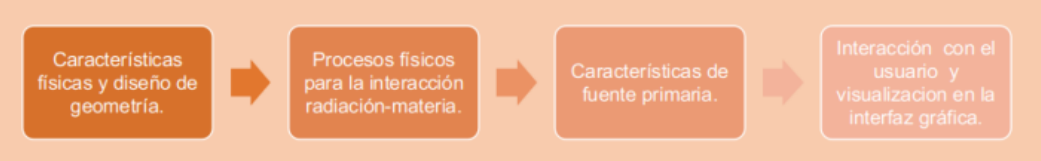
\includegraphics[width=10.3cm,height=5.6cm]{8T}
\end{center}

\newpage
 \item Analisis y resultados obtenidos.
 \end{enumerate} 
 
\begin{center}
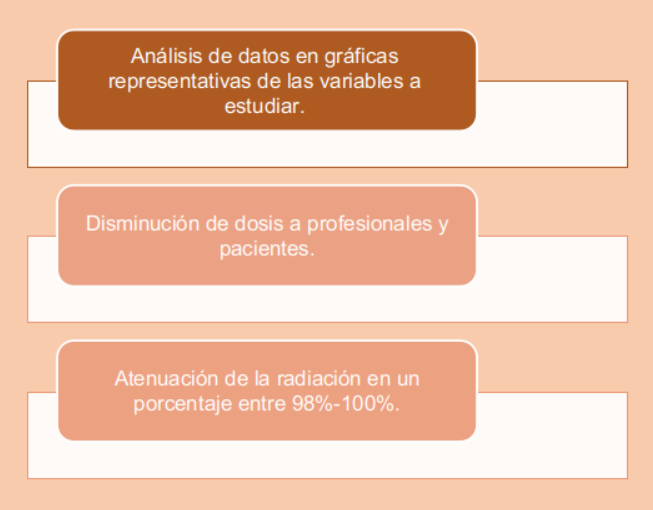
\includegraphics[width=10cm,height=7.4cm]{9T}
\end{center}
 
\section{Física del problema}

%\end{itemize}
\section{Datos Capturados}

\begin{frame}
  \frametitle{Conclusión}

  \begin{itemize}
    \item Easy to use
    \item Good results
  \end{itemize}
\end{frame}
\begin{frame}
  \frametitle{Analysis of the work}

\end{frame}

\end{document}
